\videotitle{Issues and Best Practices in NAS Research}

%-------------------------------------------------
%-------------------------------------------------


%-----------------------------------------------------------------------
\myframe{Issues in NAS Research \& Evaluations}{

	\begin{columns}[T]
	\column{0.56\textwidth}
	\begin{itemize}
	  
	  
	  \item Most NAS methods are \alert{extremely difficult to reproduce and compare} \lit{\href{https://arxiv.org/pdf/1902.07638.pdf}{Li and Talwalkar. 2019}}
	  \item For benchmarks used in almost all NAS papers:
	  \myit{
	  	\item[-] \alert{Training pipeline matters much more than neural architecture}
	  }
\bigskip
	  \onslide<2->{
		  \item The final benchmark results reported in different papers are typically \alert{incomparable}
		  \myit{
		  	\item[-] \alert{Different training code\\ (often unavailable)}
		  	\item[-] \alert{Different search spaces}
		  	\item[-] Different evaluation schemes
		  }
	  }
\medskip
	  \onslide<3->{
	  	\item[$\rightarrow$] We emphasize \alert{concepts}, not published performance numbers
	  }
	\end{itemize}
		
	\column{0.02\textwidth}
	\column{0.42\textwidth}
		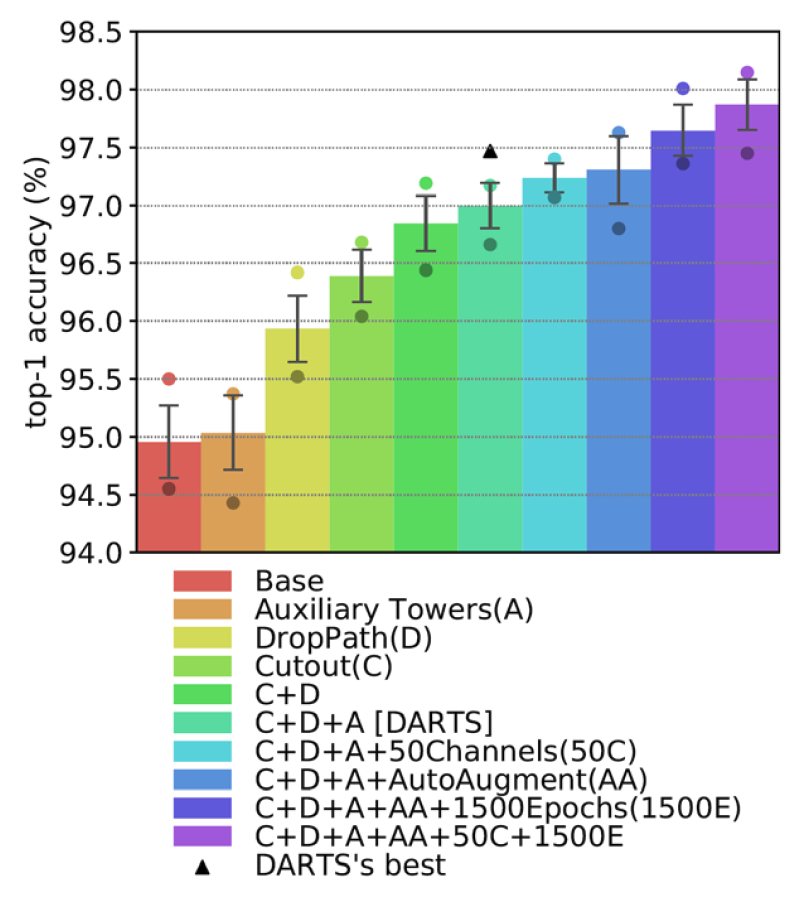
\includegraphics[width=.8\textwidth]{images/nas-eval-is-frustatingly-hard}\\
		\centering
		\lit{\href{https://openreview.net/pdf?id=HygrdpVKvr}{Yang et al. 2020}}
	\end{columns}
	
}
%-----------------------------------------------------------------------

%-----------------------------------------------------------------------
\myframe{Building a Scientific Community for NAS}{

	\myit{
	  \item \alert{Benchmarks}
	  \myit{
	  	\item[-] NAS-Bench-101 \lit{\href{https://arxiv.org/pdf/1902.09635.pdf}{Ying et al. 2019}}
	  	\item[-] NAS-Bench-201 \lit{\href{https://openreview.net/pdf?id=HJxyZkBKDr}{Dong and Yang.  2020}}
	  	\item[-] NAS-Bench-1Shot1 \lit{\href{https://openreview.net/pdf?id=SJx9ngStPH}{Zela et al. 2020}}
	  }
\medskip
\pause
	  \item \alert{Best Practice Checklist} for Scientific Research in NAS\\ \lit{\href{https://arxiv.org/pdf/1909.02453.pdf}{Lindauer and Hutter. 2020}}
\medskip
\pause
	  \item \alert{Unifying open-source implementation} of modern NAS algorithms \\ \lit{\href{https://openreview.net/pdf?id=SJx9ngStPH}{Zela et al. 2020}}
	  \myit{
	  	\item[-] Finally enables empirical comparisons without confounding factors	  	
	  }
\medskip
\pause
	  \item \alert{\href{https://sites.google.com/view/nas2020}{First NAS workshop}} at ICLR 2020
	  
	}
}
%-----------------------------------------------------------------------

%----------------------------------------------------------------------
\myframe{Best Practice Checklist for NAS Research \litw{\href{https://arxiv.org/pdf/1909.02453.pdf}{Lindauer and Hutter. 2020}}}{

\myit{
	\item Best practices for releasing code
	\myit{
		\item Code for the training pipeline used to evaluate the final architectures
		\item Hyperparameters used for the final evaluation pipeline, as well as random seeds
		\item Code for the search space
\medskip
\pause
		\item Code for your NAS method
		\item Hyperparameters for your NAS method, as well as random seeds
	} 
\pause
\bigskip
	\item Note that the easiest way to satisfy the first three is to use existing NAS benchmarks
}

\begin{center}
\begin{minipage}{0.8\textwidth}
\begin{block}{Definition: NAS Benchmark \litw{\href{https://arxiv.org/pdf/1909.02453.pdf}{Lindauer and Hutter. 2020}}}
\textit{A NAS benchmark consists of a dataset (with a predifiend training-test split), a search space, and available runnable code with pre-defined hyperparameters for training the architectures.}
\end{block}
\end{minipage}
\end{center}

}
%-----------------------------------------------------------------------

%----------------------------------------------------------------------
\myframe{Best Practice Checklist for NAS Research \litw{\href{https://arxiv.org/pdf/1909.02453.pdf}{Lindauer and Hutter. 2020}}}{

\myit{
	\item Best practices for comparing NAS methods
	\myit{
		\item For all NAS methods you compare, did you use exactly the same NAS benchmark, 
		including the same dataset (with the same training-test split), search space and code 
		for training the architectures and hyperparameters for that code?
\pause
		\item Did you control for confounding factors (different hardware, versions of DL
libraries, different runtimes for the different methods)?
\pause
		\item Did you run ablation studies?
\pause
		\item Did you use the same evaluation protocol for the methods being compared?
\pause
		\item Did you compare performance over time?
\pause
		\item Did you compare to random search?
\pause
		\item Did you perform multiple runs of your experiments and report seeds?
\pause
		\item Did you use tabular or surrogate benchmarks for in-depth evaluations?
	}
}
}
%-----------------------------------------------------------------------

%----------------------------------------------------------------------
\myframe{Best Practice Checklist for NAS Research \litw{\href{https://arxiv.org/pdf/1909.02453.pdf}{Lindauer and Hutter. 2020}}}{

\myit{
	\item Best practices for reporting important details
	\myit{
		\item Did you report how you tuned hyperparameters, and what time and resources
this required?
\pause
		\item Did you report the time for the entire end-to-end NAS method
(rather than, e.g., only for the search phase)?
\pause
		\item Did you report all the details of your experimental setup?
	}

\pause
\bigskip
	\item It might not always be possible to satisfy all these best practices, but being aware of them is the first step \ldots 


\bigskip
\pause
	\item We believe the community would benefit a lot from:
	\myit{
		\item Clean NAS benchmarks for new applications
		\myit{
			\item Including all details for the application. No need to also develop a new method.
		}
		\item Open-source library of NAS methods to compare methods without confounding factors
		\myit{
			\item First version already developed: NASlib \lit{Zela et al, under review}
		}
	}
}

}
%-----------------------------------------------------------------------


%%----------------------------------------------------------------------
%\myframe{Reproducibility crisis in NAS and the necessity of NAS benchmarks}{
%
%\myit{
%	\item \textit{\color{red}{Problem:}} Most NAS methods we saw so far are \alert{extremely difficult to reproduce and compare} (see \lit{\href{https://arxiv.org/pdf/1902.07638.pdf}{Li \& Talwalkar, 2019}; \href{https://arxiv.org/pdf/1909.02453.pdf}{Lindauer \& Hutter, 2020}}) due to:
%	\myit{
%		\item[--] Different search spaces
%		\item[--] Different training pipelines
%		\item[--] Other confounding factors, such as different hardware, different deep learning library versions, etc.
%		\item[--] Industry-scale computational resources are not accessible to everyone	
%		\item[--] No publicly available code
%	}
%\pause
%\medskip
%	\item \textit{\color{red}{Solution:}} A benchmark for NAS methods
%}
%
%
%\begin{center}
%\begin{minipage}{0.8\textwidth}
%\begin{block}{Definition: NAS Benchmark \litw{\href{https://arxiv.org/pdf/1909.02453.pdf}{Lindauer \& Hutter, 2020}}}
%\textit{A NAS benchmark consists of a dataset (with a predifiend training-test split), a search space, and available runnable code with pre-defined hyperparameters for %training the architectures.}
%\end{block}
%\end{minipage}
%\end{center}
%}
%-----------------------------------------------------------------------

%----------------------------------------------------------------------
\myframe{NAS-Bench-101: The First NAS Benchmark \litw{\href{https://arxiv.org/pdf/1902.09635.pdf}{Ying et al. 2019}}}{

\centering
\myit{
	\item Dataset: CIFAR-10, with the standard training/test split
	\item Runnable open-source code provided in Tensorflow
	\item Cell-structured search space consisting of all directed acyclic graphs (DAGs) \\ on $V$ nodes, where each possible node has $L$ operation choices.
	\pause
	\item To limit the number of architectures, NAS-Bench-101 has the following constraints:
	\myit{
		\item $L = 3$ operators:
			\begin{columns}
			\column{.18\textwidth}
			- $3 \times 3$ convolution
			\column{.18\textwidth}
			- $1 \times 1$ convolution
			\column{.2\textwidth}
			- $3 \times 3$ max-pooling			
			\end{columns}
		\item $V \leq 7$ nodes
		\item A maximum of 9 edges
	}
}

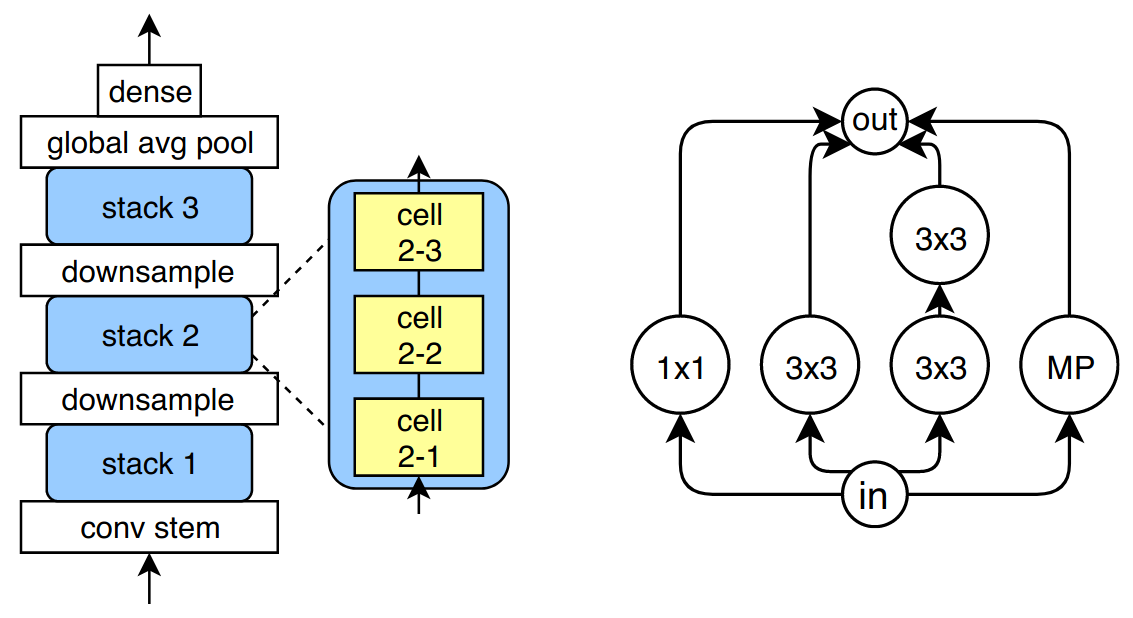
\includegraphics[width=.4\textwidth]{images/nasbench101_graph.png}

}
%-----------------------------------------------------------------------

%----------------------------------------------------------------------
\myframe{NAS-Bench-101: The First Tabular NAS Benchmark \litw{\href{https://arxiv.org/pdf/1902.09635.pdf}{Ying et al. 2019}}}{

\centering
\myit{
	\item \alert{Tabular benchmark}: we exhaustively trained and evaluated all possible models on CIFAR-10 to create a tabular (look-up table) benchmark
	\item Based on this table, anyone can now run NAS experiments in seconds without a GPU.
}

\begin{columns}
\column{.6\textwidth}
\vspace{-2.7cm}
\myit{
	\onslide<2->{
		\item Around 423k \alert{unique} cells
		\myit{
			\item[--] 4 epoch budgets: 4, 12, 36, 108
			\item[--] 3 repeats
			\item[--] around 5M trained and evaluated models
			\item[--] 120 TPU years of computation
			\item[--] the best architecture mean test accuracy: 94.32\%
			}
	}
	\medskip
	\onslide<3->{
		\item Given an architecture encoding $A$, budget $E_{stop}$ and trial number, one can query from NAS-Bench-101 the following quantities:
		\myit{
			\item[--] training/validation/test accuracy
			\item[--] training time in seconds
			\item[--] number of trainable model parameters
		}
	}
}

\column{.375\textwidth}
\onslide<2->{
	%\vspace{-3cm}
	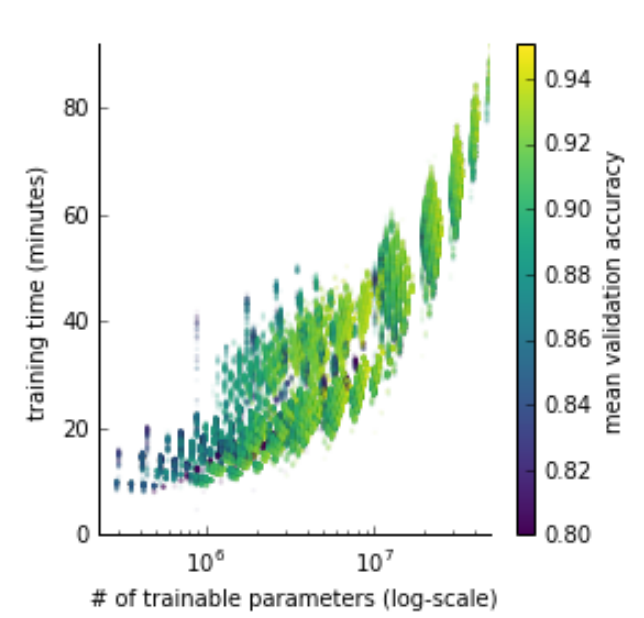
\includegraphics[width=.5\textwidth]{images/nasbench101_stat1.png}\\
	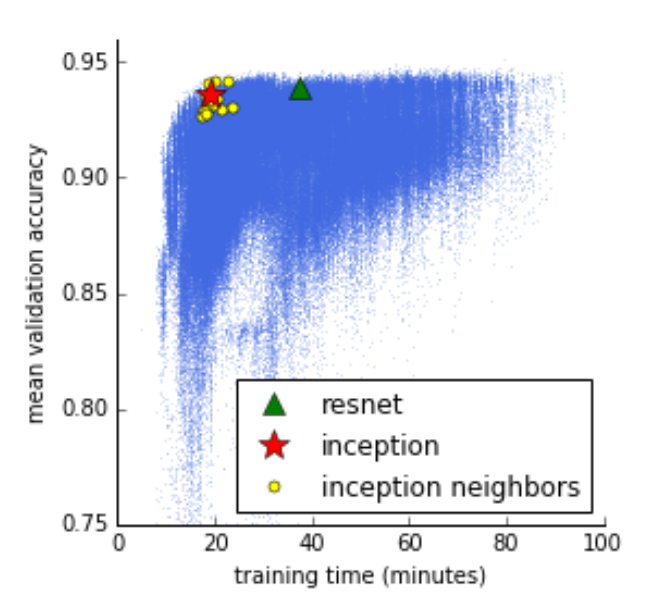
\includegraphics[width=.53\textwidth]{images/nasbench101_stat2.png}
}
\end{columns}

}
%-----------------------------------------------------------------------

%----------------------------------------------------------------------
\myframe{Evaluation of Blackbox NAS Methods on NAS-Bench-101 \litw{\href{https://arxiv.org/pdf/1902.09635.pdf}{Ying et al. 2019}}}{
	\myit{
%		\item All methods find good architectures
		\item RL outperforms random search
		\item BO and regularized evolution perform best, better than RL
	}
	\centering
	\medskip
	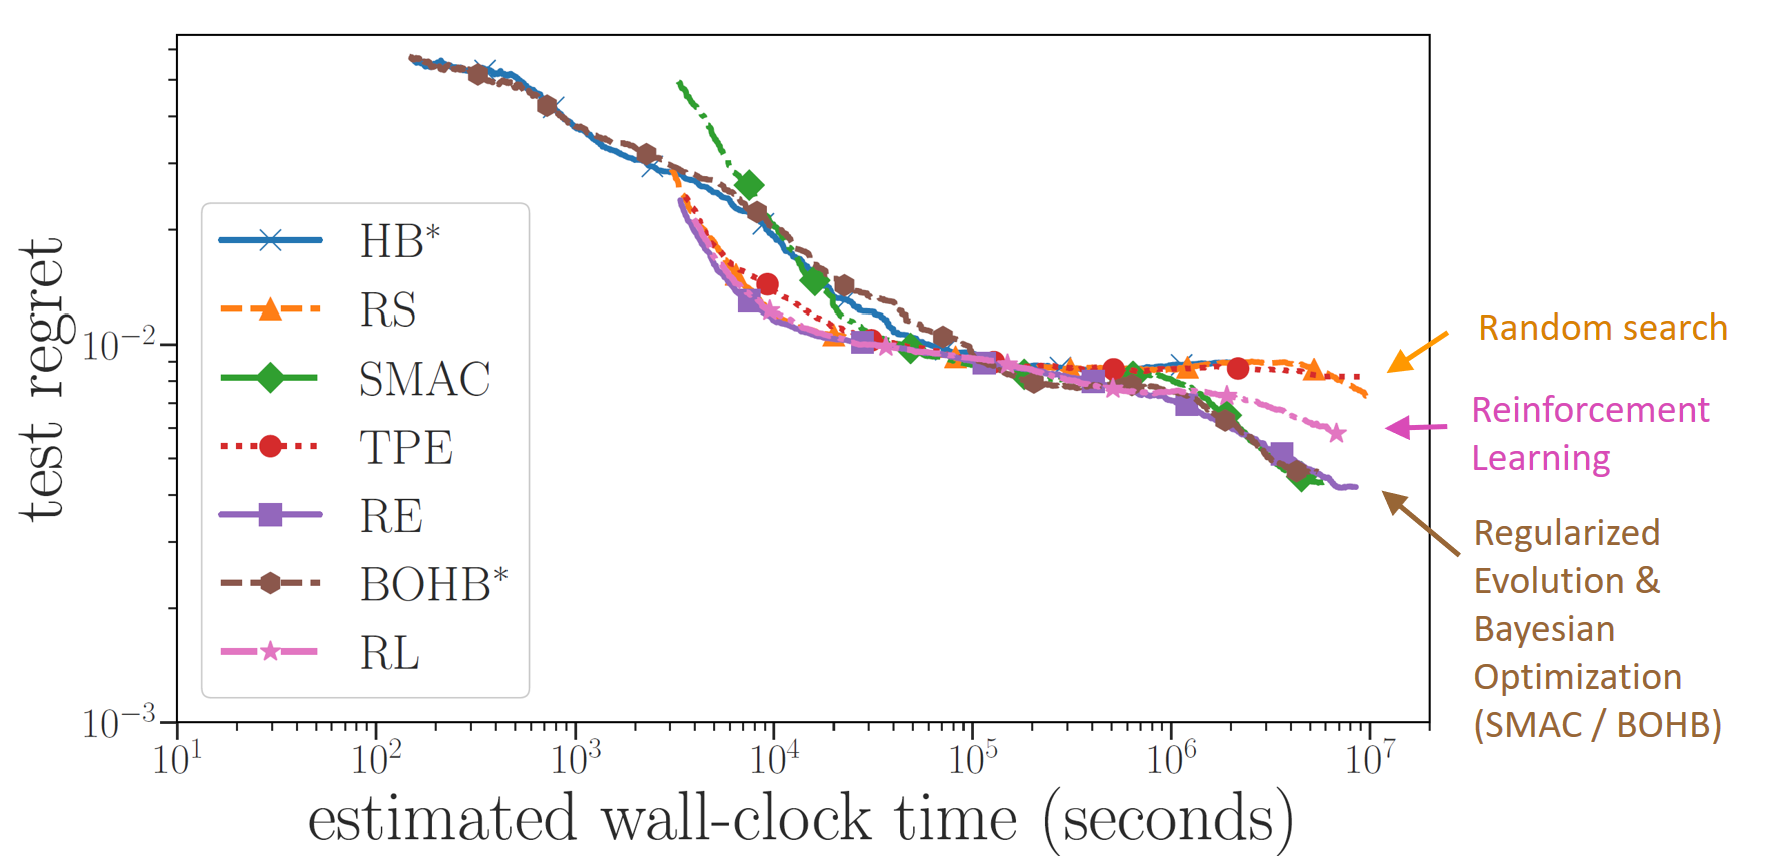
\includegraphics[width=0.64\textwidth]{images/NAS-Bench-101-results-with-labels}

\pause
	\myit{
		\item Note that the BO method SMAC \lit{\href{https://link.springer.com/chapter/10.1007/978-3-642-25566-3_40}{Hutter et al. 2011}} predated RL for \\NAS \lit{\href{https://arxiv.org/pdf/1611.01578.pdf}{Zoph and Le. 2017}} by 6 years
		\myit{
			\item[-] Only now, benchmarks like NAS-Bench-101 allow for efficient comparisons
		}
	}
}
%-----------------------------------------------------------------------

%----------------------------------------------------------------------
\myframe{Questions to Answer for Yourself / Discuss with Friends}{

	\myit{
		\item Repetition:\\ \alert{For the most common NAS search space, how important is the NAS component
		compared to the importance of the training pipeline used?}\medskip
\medskip
		\item Repetition:\\ 
		\alert{Why do we need proper benchmarking of NAS algorithms?}
\bigskip
		\item Repetition:\\
		\alert{What does a NAS benchmark consist of?}
\bigskip
		\item Repetition:\\
		\alert{List all best practices for NAS you remember.}
	}	 
}
%-----------------------------------------------------------------------